\documentclass[crop,tikz,convert={density=300,size=700x400,outext=.png}]{standalone}
\usepackage{ifthen}
\usetikzlibrary{patterns}
\usetikzlibrary{arrows.meta}

\begin{document}
%!TEX root = ../main.tex
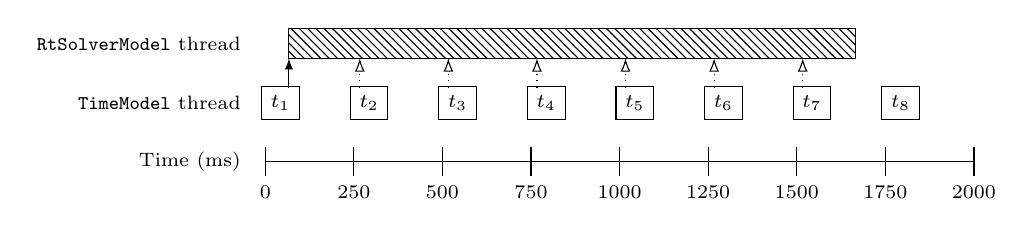
\begin{tikzpicture}[scale=.75,every node/.style={font=\scriptsize}]

\tikzset{>=latex}
\def\numTicks{8}
\def\tickWidth{1.5}

\draw (0,0) to (\numTicks*\tickWidth,0);
\node at (-.25,0) [left] {Time (ms)};
\foreach \i in {0,...,\numTicks} {
	\draw (\i*\tickWidth,.25) to (\i*\tickWidth,-.25);
	
	\node at (\i*\tickWidth,-.25) [below] {\pgfmathparse{\i*250}\pgfmathprintnumber[1000 sep={}]{\pgfmathresult}};
}

\node at (-.25,1) [left] {\texttt{TimeModel} thread};
\foreach \i in {1,...,\numTicks} {
	\draw (\i*\tickWidth-\tickWidth,.75) rectangle (\i*\tickWidth-\tickWidth+.5,1.25);	
	\node[draw,fill=white] at (\i*\tickWidth-\tickWidth-.07,1) [right] {$t_{\i}$};

	%\tikzset{arrow head=angle 60} 
	\ifthenelse{\i > 1 \AND \i < \numTicks}{
		\draw[dotted,-{Latex[fill=white]}] (\i*\tickWidth-\tickWidth+.1,1.25) to (\i*\tickWidth-\tickWidth+.1,1.75);
	}{}
}

%\foreach \i in {5,...,7} {
	%\def\vara{\pgfmathparse{\i-5}\pgfmathprintnumber[fixed]{\pgfmathresult}}
	%\node at (0,0) {\pgfmathparse{\i-5}\pgfmathprintnumber[fixed]{\pgfmathresult}}
	%\def\vara{\i-5}
%	\draw (3.5+\i*0.5,.75) rectangle (3.5+\i*.5+.5,1.25);
%	\node at (3.5+\i*.5-0.07,1) [right] {$t_{\i}$};
%}


\node at (-.25,2) [left] {\texttt{RtSolverModel} thread};

\draw[fill=white] (.4,1.75) rectangle (10,2.25);	
\draw[pattern=north west lines] (.4,1.75) rectangle (10,2.25);	
\draw[->] (.4,1.25) to (.4,1.75);



%\draw[pattern=north west lines] (3.3,1.75) rectangle (4.1,2.25);	
%\draw[->] (3.3,1.25) to (3.3,1.75);

%\draw[pattern=north west lines] (7.6,2.75) rectangle (9.5,3.25);	



\end{tikzpicture}
\end{document}